\documentclass[12pt,a4paper]{article}

%\usepackage[left=1.5cm,right=1.5cm,top=1cm,bottom=2cm]{geometry}
\usepackage[in, plain]{fullpage}
\usepackage{array}
\usepackage{../../../pas-math}
\usepackage{../../../moncours}


%\usepackage{pas-cours}
%-------------------------------------------------------------------------------
%          -Packages nécessaires pour écrire en Français et en UTF8-
%-------------------------------------------------------------------------------
\usepackage[utf8]{inputenc}
\usepackage[frenchb]{babel}
\usepackage[T1]{fontenc}
\usepackage{lmodern}
\usepackage{textcomp}



%-------------------------------------------------------------------------------

%-------------------------------------------------------------------------------
%                          -Outils de mise en forme-
%-------------------------------------------------------------------------------
\usepackage{hyperref}
\hypersetup{pdfstartview=XYZ}
%\usepackage{enumerate}
\usepackage{graphicx}
\usepackage{multicol}
\usepackage{tabularx}
\usepackage{multirow}


\usepackage{anysize} %%pour pouvoir mettre les marges qu'on veut
%\marginsize{2.5cm}{2.5cm}{2.5cm}{2.5cm}

\usepackage{indentfirst} %%pour que les premier paragraphes soient aussi indentés
\usepackage{verbatim}
\usepackage{enumitem}
\usepackage[usenames,dvipsnames,svgnames,table]{xcolor}

\usepackage{variations}

%-------------------------------------------------------------------------------


%-------------------------------------------------------------------------------
%                  -Nécessaires pour écrire des mathématiques-
%-------------------------------------------------------------------------------
\usepackage{amsfonts}
\usepackage{amssymb}
\usepackage{amsmath}
\usepackage{amsthm}
\usepackage{tikz}
\usepackage{xlop}
%-------------------------------------------------------------------------------



%-------------------------------------------------------------------------------


%-------------------------------------------------------------------------------
%                    - Mise en forme avancée
%-------------------------------------------------------------------------------

\usepackage{ifthen}
\usepackage{ifmtarg}


\newcommand{\ifTrue}[2]{\ifthenelse{\equal{#1}{true}}{#2}{$\qquad \qquad$}}

%-------------------------------------------------------------------------------

%-------------------------------------------------------------------------------
%                     -Mise en forme d'exercices-
%-------------------------------------------------------------------------------
%\newtheoremstyle{exostyle}
%{\topsep}% espace avant
%{\topsep}% espace apres
%{}% Police utilisee par le style de thm
%{}% Indentation (vide = aucune, \parindent = indentation paragraphe)
%{\bfseries}% Police du titre de thm
%{.}% Signe de ponctuation apres le titre du thm
%{ }% Espace apres le titre du thm (\newline = linebreak)
%{\thmname{#1}\thmnumber{ #2}\thmnote{. \normalfont{\textit{#3}}}}% composants du titre du thm : \thmname = nom du thm, \thmnumber = numéro du thm, \thmnote = sous-titre du thm

%\theoremstyle{exostyle}
%\newtheorem{exercice}{Exercice}
%
%\newenvironment{questions}{
%\begin{enumerate}[\hspace{12pt}\bfseries\itshape a.]}{\end{enumerate}
%} %mettre un 1 à la place du a si on veut des numéros au lieu de lettres pour les questions 
%-------------------------------------------------------------------------------

%-------------------------------------------------------------------------------
%                    - Mise en forme de tableaux -
%-------------------------------------------------------------------------------

\renewcommand{\arraystretch}{1.7}

\setlength{\tabcolsep}{1.2cm}

%-------------------------------------------------------------------------------



%-------------------------------------------------------------------------------
%                    - Racourcis d'écriture -
%-------------------------------------------------------------------------------

% Angles orientés (couples de vecteurs)
\newcommand{\aopp}[2]{(\vec{#1}, \vec{#2})} %Les deuc vecteurs sont positifs
\newcommand{\aopn}[2]{(\vec{#1}, -\vec{#2})} %Le second vecteur est négatif
\newcommand{\aonp}[2]{(-\vec{#1}, \vec{#2})} %Le premier vecteur est négatif
\newcommand{\aonn}[2]{(-\vec{#1}, -\vec{#2})} %Les deux vecteurs sont négatifs

%Ensembles mathématiques
\newcommand{\naturels}{\mathbb{N}} %Nombres naturels
\newcommand{\relatifs}{\mathbb{Z}} %Nombres relatifs
\newcommand{\rationnels}{\mathbb{Q}} %Nombres rationnels
\newcommand{\reels}{\mathbb{R}} %Nombres réels
\newcommand{\complexes}{\mathbb{C}} %Nombres complexes


%Intégration des parenthèses aux cosinus
\newcommand{\cosP}[1]{\cos\left(#1\right)}
\newcommand{\sinP}[1]{\sin\left(#1\right)}


%Probas stats
\newcommand{\stat}{statistique}
\newcommand{\stats}{statistiques}
%-------------------------------------------------------------------------------

%-------------------------------------------------------------------------------
%                    - Mise en page -
%-------------------------------------------------------------------------------

\newcommand{\twoCol}[1]{\begin{multicols}{2}#1\end{multicols}}


\setenumerate[1]{font=\bfseries,label=\textit{\alph*})}
\setenumerate[2]{font=\bfseries,label=\arabic*)}


%-------------------------------------------------------------------------------
%                    - Elements cours -
%-------------------------------------------------------------------------------





%\makeatletter
%\renewcommand*{\@seccntformat}[1]{\csname the#1\endcsname\hspace{0.1cm}}
%\makeatother


%\author{Olivier FINOT}
\date{}
\title{Information chiffrée }

%\newcommand{\disp}{false}

\lhead{CH2 : Suites numériques}
\rhead{O. FINOT}
%
%\rfoot{Page \thepage}
\begin{document}
%\maketitle

\chap[num=2, color=red]{Suites numériques}{Olivier FINOT, \today }

\begin{myobj}
	\begin{itemize}
		
		\item Construire le symétrique d’un point ou d'une figure par rapport à une droite à la main où à l’aide d’un logiciel;
		\item Construire le symétrique d’un point ou d'une figure par rapport à un point, à la main où à l’aide d’un logiciel;
		\item Utiliser les propriétés de la symétrie axiale ou centrale;
		\item Identifier des symétries dans des figures.		
	\end{itemize}
\end{myobj}

\begin{mycomp}
	\begin{itemize}
		\item \kw{Chercher (Ch2)} :  s’engager    dans    une    démarche    scientifique, observer, questionner, manipuler, expérimenter (sur une feuille de papier, avec des objets, à l’aide de logiciels), émettre des hypothèses, chercher des exemples ou des contre-exemples, simplifier ou particulariser une situation, émettre une conjecture ;
		\item \kw{Raisonner (Ra3)} :  démontrer : utiliser un raisonnement logique et des règles établies (propriétés, théorèmes, formules) pour parvenir à une conclusion ;
		\item \kw{Communiquer (Co2)} :  expliquer à l’oral ou à l’écrit (sa démarche, son raisonnement, un calcul, un protocole   de   construction   géométrique, un algorithme), comprendre les explications d’un autre et argumenter dans l’échange ; 
		
	\end{itemize}
\end{mycomp}




\section{Suite numérique}

\begin{mydef}
	Une \kw{suite numérique} est constituée de \kw{plusieurs nombres rangés dans un certain ordre}. Ces nombres sont les \kw{termes} de la suite. Le premier terme de la suite est noté $u_1$ (ou $u_0$), le deuxième $u_2$ (ou $u_1$), $u_n$ est le n-ième (ou n+1-ième). Le terme suivant est noté $u_{n+1}$.
	
\end{mydef}

\begin{myex}
	On considère le prix d'un litre de gazole relevé dans une même station au premier janvier entre 1999 et 2008.
	\begin{align*}
		0,62 \:;\: 0,95 \:;\: 0,82 \:; \:0,78 \:;\: 0,81 \:;\: 0,80 \:;\: 0,92 \:;\: 1,05 \:;\: 1,01 \:; \:1,20
	\end{align*}
	
	Le premier terme est $0,62$ ; le deuxième terme est $0,95$ ; le troisième est $0,82$ , ...
	On a
	$u_1=0,62$, $u_2=0,95$, $u_3=0,82$ , ...
\end{myex}

\section{Suites arithmétiques}


\begin{myact}{La suite des nombres impairs}
	On considère la suite des nombres impairs, 1, 3, 5, 7, ..., que l'on note successivement $u_1$, $u_2$, $u_3$, $u_4$...
	Donc $u_1=1$, $u_2=3$, $u_3=5$...\\
	
	\begin{enumerate}
		\item Compléter : $u_4=.....$, $u_? =15$, $u_{10}=......$.
		\item Quel est le premier terme de la suite ?
		\item Comment passe-t-on d'un terme au suivant ?
		\item $n$ est est nombre entier positif non nul, on s'intéresse au terme de rang $n$ (donc le $n^{ième}$ nombre impair). Exprimer $u_{n+1}$ en fonction de $u_n$.
		\item Exprimer $u_n$ en fonction de $n$.
		\item Calculer $u_{100}$, $u_{150}$, $u_{1000}$.
	\end{enumerate}
	
\end{myact}

\subsection{Définition}



\begin{mybilan}

Une \kw{suite arithmétique} est une suite de nombres, où chaque terme, à partir du deuxième est obtenu en ajoutant au précédent un même nombre, la \kw{raison} de la suite (notée $r$).	
		On note :
		\kw{{\LARGE \begin{align*}
					u_{n+1} = u_n + r 
				\end{align*}}}
			
\end{mybilan}

\begin{myex}
	\begin{enumerate}
		\item La suite $(u_n)$ des entiers naturels : 
		
		On a $u_0$ = 0; $u_1$ = 1; $u_2$ = 2; $u_3$ = 3 ...
		
		C'est une suite arithmétique de premier terme $u_0$ = 0 et de raison 1; \\ $u_{n+1} = u_n + 1 $
		
		\item La suite $(v_n)$ des entiers naturels pairs: 
		
		On a $v_0$ = 0; $v_1$ = 2; $v_2$ = 4; $v_3$ = 6 ...
		
		C'est une suite arithmétique de premier terme $v_0$ = 0 et de raison 2,\\ $v_{n+1} = v_n + 2 $
	\end{enumerate}
\end{myex}


\begin{myrem}
	\begin{itemize}
		\item Une suite arithmétique est définie par son terme initial et sa raison "$r$"
		
		\item Pour démontrer qu'une suite est arithmétique, il suffit de vérifier que la différence entre deux termes consécutifs ($u_{n+1}-u_n$) est constante; cette constante est la raison "$r$".
	\end{itemize}
\end{myrem}

\subsection{Expression de $u_n$ en fonction de $n$}

\begin{mybilan}
	Dans une suite arithmétique de raison $r$, le terme $u_n$ est obtenu à partir du premier terme par la relation :
	\begin{itemize}
		\item \kw{$u_n = u_0 + nr$} (lorsque le terme initial est $u_0$) 
		\item \kw{$u_n = u_1 + (n-1)r$} (lorsque le terme initial est $u_1$)
	\end{itemize}
	
	\begin{multicols}{2}
		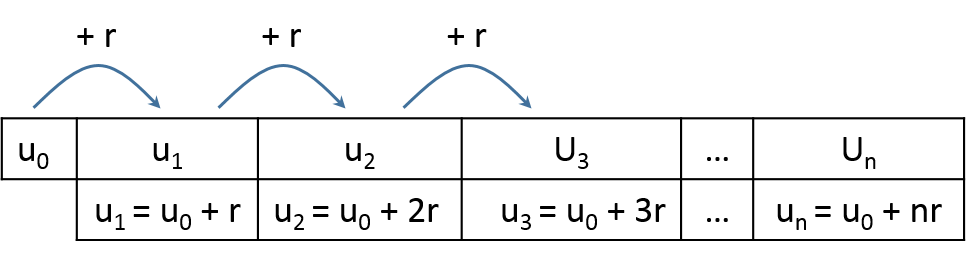
\includegraphics[scale=0.4]{./img/arith1}
		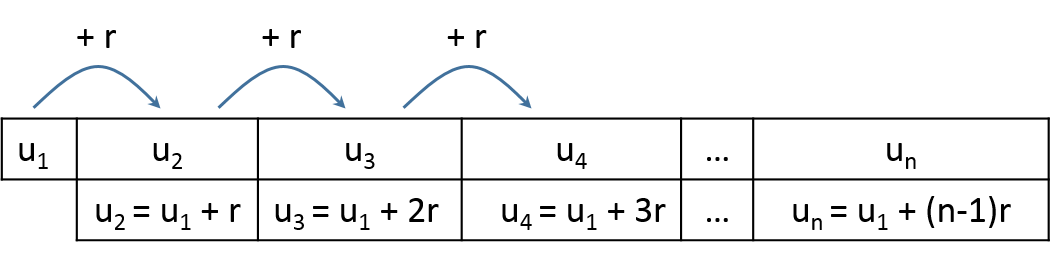
\includegraphics[scale=0.4]{./img/arith2}
	\end{multicols}
\end{mybilan}


\begin{myex}
	$(u_n)$ est la suite des entiers naturels impairs :
	
	On a $u_0$ = 1; $u_1$ = 3; $u_2$ = 5; $u_3$ = 7 ...
	
	C'est une suite arithmétique de premier terme $u_0$ = 1 et de raison 2.
	
	Calcul du centième nombre impair :
	 On calcule donc $u_{99}$
	 
	 \begin{eqnarray*}
	 	u_{99} & = & u_0 + 99 \times r \\
				& = & 1 + 99 \times 2 \\
				& = & 1 + 198 \\
		u_{99}	& = & 199	 	
	 \end{eqnarray*}
 
 Le centième nombre impair est égal à 199.
 
 
 Pour cette suite on a :
	 \begin{eqnarray*}
	 	 u_{n} & = & u_0 + n \times r \\
		soit \quad u_n & = & 1 + n \times 2 \\
	 	 u_n & = & 1 + 2n \\
	 	 u_{99}	& = & 2n + 1	 	
	 \end{eqnarray*}
 
\end{myex}
\subsection{Représentation graphique}	

\begin{myex}
	La suite des nombres impairs est définie par : $u_{n} = 2n +1$.
	On représente graphiquement les termes de la suite :
	
	\begin{multicols}{2}
			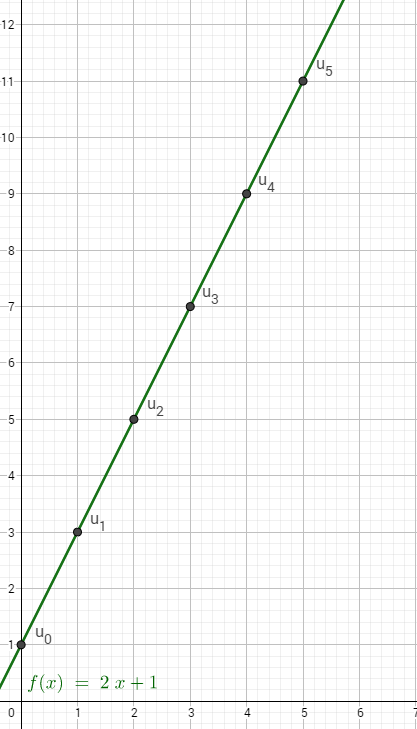
\includegraphics[scale=0.5]{img/arith}
			
			\begin{itemize}
				\item La représentation graphique de la suite $(u_n)$ est consituée de points alignés sur la droite d'équation $y=2x+1$.
				\item Le premier terme $u_0=1$ est l'ordonnée à l'origine de la droite et la raison $r=2$ est son coefficient directeur
			\end{itemize}
			
	\end{multicols}

\end{myex}	

\begin{mybilan}{Représentation graphique}
	La représentation grpahique d'une suite arithmétique est constituée de points alignés. Il y a le même écart entre chaque couple de points consécutifs.
\end{mybilan}
\section{Suites géométrique}

\begin{myact}{La suite des nombres impairs}
	On considère la suite des nombres impairs, 1, 3, 5, 7, ..., que l'on note successivement $u_1$, $u_2$, $u_3$, $u_4$...
	Donc $u_1=1$, $u_2=3$, $u_3=5$...\\
	
	\begin{enumerate}
		\item Compléter : $u_4=.....$, $u_? =15$, $u_{10}=......$.
		\item Quel est le premier terme de la suite ?
		\item Comment passe-t-on d'un terme au suivant ?
		\item $n$ est est nombre entier positif non nul, on s'intéresse au terme de rang $n$ (donc le $n^{ième}$ nombre impair). Exprimer $u_{n+1}$ en fonction de $u_n$.
		\item Exprimer $u_n$ en fonction de $n$.
		\item Calculer $u_{100}$, $u_{150}$, $u_{1000}$.
	\end{enumerate}
	
\end{myact}


\begin{mybilan}
	\begin{itemize}
		
		\item Une \kw{suite géométrique} est une suite de nombres, où chaque terme, à partir du deuxième est obtenu multipliant le précédent par un même nombre, la \kw{raison} de la suite (notée $q$).	
		On note :
		\kw{{\LARGE \begin{align*}
					u_{n+1} = u_n \times q 
		\end{align*}}}
		
		\item 		Dans une suite géométrique de raison $q$, le terme $u_n$ est obtenu à partir du premier terme par la relation :
		\begin{itemize}
			\item \kw{$u_n = u_0 \times q^n$} (lorsque le terme initial est $u_0$) 
			\item \kw{$u_n = u_1 \times q^{n-1}$} (lorsque le terme initial est $u_1$)
		\end{itemize}
		
		\begin{multicols}{2}
			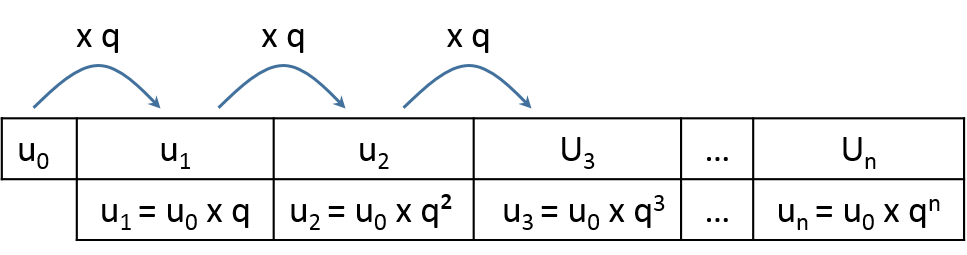
\includegraphics[scale=0.4]{./img/geo1}
			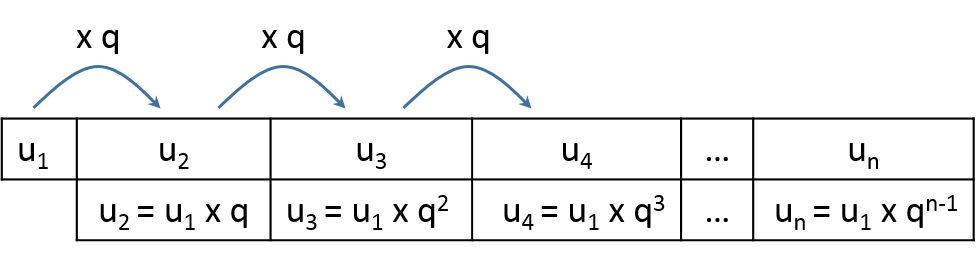
\includegraphics[scale=0.4]{./img/geo2}
		\end{multicols}
	\end{itemize}
\end{mybilan}	
\end{document}